\documentclass{article}
\usepackage{ifthen}
\usepackage{amssymb}
\usepackage{multicol}
\usepackage{graphicx}
\usepackage[absolute]{textpos}
\usepackage{amsmath, amscd, amssymb, amsthm, latexsym}
% \usepackage[noload]{qtree}
%\usepackage{xspace,rotating,calligra,dsfont,ifthen}
\usepackage{xspace,rotating,dsfont,ifthen}
\usepackage[spanish,activeacute]{babel}
\usepackage[utf8]{inputenc}
\usepackage{pgfpages}
\usepackage{pgf,pgfarrows,pgfnodes,pgfautomata,pgfheaps,xspace,dsfont}
\usepackage{listings}
\usepackage{multicol}
\usepackage{todonotes}
\usepackage{url}
\usepackage{float}
\usepackage{framed,mdframed}
\usepackage{cancel}

\usepackage[strict]{changepage}


\makeatletter


\newcommand\hfrac[2]{\genfrac{}{}{0pt}{}{#1}{#2}} %\hfrac{}{} es un \frac sin la linea del medio

\newcommand\Wider[2][3em]{% \Wider[3em]{} reduce los m\'argenes
\makebox[\linewidth][c]{%
  \begin{minipage}{\dimexpr\textwidth+#1\relax}
  \raggedright#2
  \end{minipage}%
  }%
}


\@ifclassloaded{beamer}{%
  \newcommand{\tocarEspacios}{%
    \addtolength{\leftskip}{4em}%
    \addtolength{\parindent}{-3em}%
  }%
}
{%
  \usepackage[top=1cm,bottom=2cm,left=1cm,right=1cm]{geometry}%
  \usepackage{color}%
  \newcommand{\tocarEspacios}{%
    \addtolength{\leftskip}{3em}%
    \setlength{\parindent}{0em}%
  }%
}

\newcommand{\encabezadoDeProc}[4]{%
  % Ponemos la palabrita problema en tt
%  \noindent%
  {\normalfont\bfseries\ttfamily proc}%
  % Ponemos el nombre del problema
  \ %
  {\normalfont\ttfamily #2}%
  \
  % Ponemos los parametros
  (#3)%
  \ifthenelse{\equal{#4}{}}{}{%
  \ =\ %
  % Ponemos el nombre del resultado
  {\normalfont\ttfamily #1}%
  % Por ultimo, va el tipo del resultado
  \ : #4}
}

\newcommand{\encabezadoDeTipo}[2]{%
  % Ponemos la palabrita tipo en tt
  {\normalfont\bfseries\ttfamily tipo}%
  % Ponemos el nombre del tipo
  \ %
  {\normalfont\ttfamily #2}%
  \ifthenelse{\equal{#1}{}}{}{$\langle$#1$\rangle$}
}

% Primero definiciones de cosas al estilo title, author, date

\def\materia#1{\gdef\@materia{#1}}
\def\@materia{No especifi\'o la materia}
\def\lamateria{\@materia}

\def\cuatrimestre#1{\gdef\@cuatrimestre{#1}}
\def\@cuatrimestre{No especifi\'o el cuatrimestre}
\def\elcuatrimestre{\@cuatrimestre}

\def\anio#1{\gdef\@anio{#1}}
\def\@anio{No especifi\'o el anio}
\def\elanio{\@anio}

\def\fecha#1{\gdef\@fecha{#1}}
\def\@fecha{\today}
\def\lafecha{\@fecha}

\def\nombre#1{\gdef\@nombre{#1}}
\def\@nombre{No especific'o el nombre}
\def\elnombre{\@nombre}

\def\practicas#1{\gdef\@practica{#1}}
\def\@practica{No especifi\'o el n\'umero de pr\'actica}
\def\lapractica{\@practica}


% Esta macro convierte el numero de cuatrimestre a palabras
\newcommand{\cuatrimestreLindo}{
  \ifthenelse{\equal{\elcuatrimestre}{1}}
  {Primer cuatrimestre}
  {\ifthenelse{\equal{\elcuatrimestre}{2}}
  {Segundo cuatrimestre}
  {Verano}}
}


\newcommand{\depto}{{UBA -- Facultad de Ciencias Exactas y Naturales --
      Departamento de Computaci\'on}}

\newcommand{\titulopractica}{
  \centerline{\depto}
  \vspace{1ex}
  \centerline{{\Large\lamateria}}
  \vspace{0.5ex}
  \centerline{\cuatrimestreLindo de \elanio}
  \vspace{2ex}
  \centerline{{\huge Pr\'actica \lapractica -- \elnombre}}
  \vspace{5ex}
  \arreglarincisos
  \newcounter{ejercicio}
  \newenvironment{ejercicio}{\stepcounter{ejercicio}\textbf{Ejercicio
      \theejercicio}%
    \renewcommand\@currentlabel{\theejercicio}%
  }{\vspace{0.2cm}}
}


\newcommand{\titulotp}{
  \centerline{\depto}
  \vspace{1ex}
  \centerline{{\Large\lamateria}}
  \vspace{0.5ex}
  \centerline{\cuatrimestreLindo de \elanio}
  \vspace{0.5ex}
  \centerline{\lafecha}
  \vspace{2ex}
  \centerline{{\huge\elnombre}}
  \vspace{5ex}
}


%practicas
\newcommand{\practica}[2]{%
    \title{Pr\'actica #1 \\ #2}
    \author{Algoritmos y Estructuras de Datos I}
    \date{Segundo Cuatrimestre 2019}

    \maketitlepractica{#1}{#2}
}

\newcommand \maketitlepractica[2] {%
\begin{center}
\begin{tabular}{r cr}
 \begin{tabular}{c}
{\large\bf\textsf{\ Algoritmos y Estructuras de Datos I\ }}\\
Primer Cuatrimestre 2021\\
\title{\normalsize Gu\'ia Pr\'actica #1 \\ \textbf{#2}}\\
\@title
\end{tabular} &
\begin{tabular}{@{} p{1.6cm} @{}}
\includegraphics[width=1.6cm]{logodpt.jpg}
\end{tabular} &
\begin{tabular}{l @{}}
 \emph{Departamento de Computaci\'on} \\
 \emph{Facultad de Ciencias Exactas y Naturales} \\
 \emph{Universidad de Buenos Aires} \\
\end{tabular}
\end{tabular}
\end{center}

\bigskip
}


% Símbolos varios

\newcommand{\nat}{\ensuremath{\mathds{N}}}
\newcommand{\ent}{\ensuremath{\mathds{Z}}}
\newcommand{\float}{\ensuremath{\mathds{R}}}
\newcommand{\bool}{\ensuremath{\mathsf{Bool}}}
\newcommand{\True}{\ensuremath{\mathrm{true}}}
\newcommand{\False}{\ensuremath{\mathrm{false}}}
\newcommand{\Then}{\ensuremath{\rightarrow}}
\newcommand{\Iff}{\ensuremath{\leftrightarrow}}
\newcommand{\implica}{\ensuremath{\longrightarrow}}
\newcommand{\IfThenElse}[3]{\ensuremath{\mathsf{if}\ #1\ \mathsf{then}\ #2\ \mathsf{else}\ #3\ \mathsf{fi}}}
\newcommand{\In}{\textsf{in }}
\newcommand{\Out}{\textsf{out }}
\newcommand{\Inout}{\textsf{inout }}
\newcommand{\yLuego}{\land _L}
\newcommand{\oLuego}{\lor _L}
\newcommand{\implicaLuego}{\implica _L}
\newcommand{\cuantificador}[5]{%
	\ensuremath{(#2 #3: #4)\ (%
		\ifthenelse{\equal{#1}{unalinea}}{
			#5
		}{
			$ % exiting math mode
			\begin{adjustwidth}{+2em}{}
			$#5$%
			\end{adjustwidth}%
			$ % entering math mode
		}
	)}
}

\newcommand{\existe}[4][]{%
	\cuantificador{#1}{\exists}{#2}{#3}{#4}
}
\newcommand{\paraTodo}[4][]{%
	\cuantificador{#1}{\forall}{#2}{#3}{#4}
}

% Símbolo para marcar los ejercicios importantes (estrellita)
\newcommand\importante{\raisebox{0.5pt}{\ensuremath{\bigstar}}}


\newcommand{\rango}[2]{[#1\twodots#2]}
\newcommand{\comp}[2]{[\,#1\,|\,#2\,]}

\newcommand{\rangoac}[2]{(#1\twodots#2]}
\newcommand{\rangoca}[2]{[#1\twodots#2)}
\newcommand{\rangoaa}[2]{(#1\twodots#2)}

%ejercicios
\newtheorem{exercise}{Ejercicio}
\newenvironment{ejercicio}[1][]{\begin{exercise}#1\rm}{\end{exercise} \vspace{0.2cm}}
\newenvironment{items}{\begin{enumerate}[a)]}{\end{enumerate}}
\newenvironment{subitems}{\begin{enumerate}[i)]}{\end{enumerate}}
\newcommand{\sugerencia}[1]{\noindent \textbf{Sugerencia:} #1}

\lstnewenvironment{code}{
    \lstset{% general command to set parameter(s)
        language=C++, basicstyle=\small\ttfamily, keywordstyle=\slshape,
        emph=[1]{tipo,usa}, emphstyle={[1]\sffamily\bfseries},
        morekeywords={tint,forn,forsn},
        basewidth={0.47em,0.40em},
        columns=fixed, fontadjust, resetmargins, xrightmargin=5pt, xleftmargin=15pt,
        flexiblecolumns=false, tabsize=2, breaklines, breakatwhitespace=false, extendedchars=true,
        numbers=left, numberstyle=\tiny, stepnumber=1, numbersep=9pt,
        frame=l, framesep=3pt,
    }
   \csname lst@SetFirstLabel\endcsname}
  {\csname lst@SaveFirstLabel\endcsname}


%tipos basicos
\newcommand{\rea}{\ensuremath{\mathsf{Float}}}
\newcommand{\cha}{\ensuremath{\mathsf{Char}}}
\newcommand{\str}{\ensuremath{\mathsf{String}}}

\newcommand{\mcd}{\mathrm{mcd}}
\newcommand{\prm}[1]{\ensuremath{\mathsf{prm}(#1)}}
\newcommand{\sgd}[1]{\ensuremath{\mathsf{sgd}(#1)}}

\newcommand{\tuple}[2]{\ensuremath{#1 \times #2}}

%listas
\newcommand{\TLista}[1]{\ensuremath{seq \langle #1\rangle}}
\newcommand{\lvacia}{\ensuremath{[\ ]}}
\newcommand{\lv}{\ensuremath{[\ ]}}
\newcommand{\longitud}[1]{\ensuremath{|#1|}}
\newcommand{\cons}[1]{\ensuremath{\mathsf{addFirst}}(#1)}
\newcommand{\indice}[1]{\ensuremath{\mathsf{indice}}(#1)}
\newcommand{\conc}[1]{\ensuremath{\mathsf{concat}}(#1)}
\newcommand{\cab}[1]{\ensuremath{\mathsf{head}}(#1)}
\newcommand{\cola}[1]{\ensuremath{\mathsf{tail}}(#1)}
\newcommand{\sub}[1]{\ensuremath{\mathsf{subseq}}(#1)}
\newcommand{\en}[1]{\ensuremath{\mathsf{en}}(#1)}
\newcommand{\cuenta}[2]{\mathsf{cuenta}\ensuremath{(#1, #2)}}
\newcommand{\suma}[1]{\mathsf{suma}(#1)}
\newcommand{\twodots}{\ensuremath{\mathrm{..}}}
\newcommand{\masmas}{\ensuremath{++}}
\newcommand{\matriz}[1]{\TLista{\TLista{#1}}}

\newcommand{\seqchar}{\TLista{\cha}}


% Acumulador
\newcommand{\acum}[1]{\ensuremath{\mathsf{acum}}(#1)}
\newcommand{\acumselec}[3]{\ensuremath{\mathrm{acum}(#1 |  #2, #3)}}

% \selector{variable}{dominio}
\newcommand{\selector}[2]{#1~\ensuremath{\leftarrow}~#2}
\newcommand{\selec}{\ensuremath{\leftarrow}}

\newcommand{\pred}[3]{%
    {\normalfont\bfseries\ttfamily\noindent pred }%
    {\normalfont\ttfamily #1}%
    \ifthenelse{\equal{#2}{}}{}{\ (#2) }%
    \{%
    \begin{adjustwidth}{+2em}{}
      \ensuremath{#3}
    \end{adjustwidth}
    \}%
    {\normalfont\bfseries\,\par}%
}

\newenvironment{proc}[4][res]{%

  % El parametro 1 (opcional) es el nombre del resultado
  % El parametro 2 es el nombre del problema
  % El parametro 3 son los parametros
  % El parametro 4 es el tipo del resultado
  % Preambulo del ambiente problema
  % Tenemos que definir los comandos requiere, asegura, modifica y aux
  \newcommand{\pre}[2][]{%
    {\normalfont\bfseries\ttfamily Pre}%
    \ifthenelse{\equal{##1}{}}{}{\ {\normalfont\ttfamily ##1} :}\ %
    \{\ensuremath{##2}\}%
    {\normalfont\bfseries\,\par}%
  }
  \newcommand{\post}[2][]{%
    {\normalfont\bfseries\ttfamily Post}%
    \ifthenelse{\equal{##1}{}}{}{\ {\normalfont\ttfamily ##1} :}\
    \{\ensuremath{##2}\}%
    {\normalfont\bfseries\,\par}%
  }
  \renewcommand{\aux}[4]{%
    {\normalfont\bfseries\ttfamily aux\ }%
    {\normalfont\ttfamily ##1}%
    \ifthenelse{\equal{##2}{}}{}{\ (##2)}\ : ##3\, = \ensuremath{##4}%
    {\normalfont\bfseries\,;\par}%
  }
  \renewcommand{\pred}[3]{%
    {\normalfont\bfseries\ttfamily pred }%
    {\normalfont\ttfamily ##1}%
    \ifthenelse{\equal{##2}{}}{}{\ (##2) }%
    \{%
    \begin{adjustwidth}{+5em}{}
      \ensuremath{##3}
    \end{adjustwidth}
    \}%
    {\normalfont\bfseries\,\par}%
  }

  \newcommand{\res}{#1}
  \vspace{1ex}
  \noindent
  \encabezadoDeProc{#1}{#2}{#3}{#4}
  % Abrimos la llave
  \{\par%
  \tocarEspacios
}
% Ahora viene el cierre del ambiente problema
{
  % Cerramos la llave
  \noindent\}
  \vspace{1ex}
}


\newcommand{\aux}[4]{%
    {\normalfont\bfseries\ttfamily\noindent aux\ }%
    {\normalfont\ttfamily #1}%
    \ifthenelse{\equal{#2}{}}{}{\ (#2)}\ : #3\, = \ensuremath{#4}%
    {\normalfont\bfseries\,;\par}%
}


% \newcommand{\pre}[1]{\textsf{pre}\ensuremath{(#1)}}

\newcommand{\procnom}[1]{\textsf{#1}}
\newcommand{\procil}[3]{\textsf{proc #1}\ensuremath{(#2) = #3}}
\newcommand{\procilsinres}[2]{\textsf{proc #1}\ensuremath{(#2)}}
\newcommand{\preil}[2]{\textsf{Pre #1: }\ensuremath{#2}}
\newcommand{\postil}[2]{\textsf{Post #1: }\ensuremath{#2}}
\newcommand{\auxil}[2]{\textsf{fun }\ensuremath{#1 = #2}}
\newcommand{\auxilc}[4]{\textsf{fun }\ensuremath{#1( #2 ): #3 = #4}}
\newcommand{\auxnom}[1]{\textsf{fun }\ensuremath{#1}}
\newcommand{\auxpred}[3]{\textsf{pred }\ensuremath{#1( #2 ) \{ #3 \}}}

\newcommand{\comentario}[1]{{/*\ #1\ */}}

\newcommand{\nom}[1]{\ensuremath{\mathsf{#1}}}


% En las practicas/parciales usamos numeros arabigos para los ejercicios.
% Aca cambiamos los enumerate comunes para que usen letras y numeros
% romanos
\newcommand{\arreglarincisos}{%
  \renewcommand{\theenumi}{\alph{enumi}}
  \renewcommand{\theenumii}{\roman{enumii}}
  \renewcommand{\labelenumi}{\theenumi)}
  \renewcommand{\labelenumii}{\theenumii)}
}



%%%%%%%%%%%%%%%%%%%%%%%%%%%%%% PARCIAL %%%%%%%%%%%%%%%%%%%%%%%%
\let\@xa\expandafter
\newcommand{\tituloparcial}{\centerline{\depto -- \lamateria}
  \centerline{\elnombre -- \lafecha}%
  \setlength{\TPHorizModule}{10mm} % Fija las unidades de textpos
  \setlength{\TPVertModule}{\TPHorizModule} % Fija las unidades de
                                % textpos
  \arreglarincisos
  \newcounter{total}% Este contador va a guardar cuantos incisos hay
                    % en el parcial. Si un ejercicio no tiene incisos,
                    % cuenta como un inciso.
  \newcounter{contgrilla} % Para hacer ciclos
  \newcounter{columnainicial} % Se van a usar para los cline cuando un
  \newcounter{columnafinal}   % ejercicio tenga incisos.
  \newcommand{\primerafila}{}
  \newcommand{\segundafila}{}
  \newcommand{\rayitas}{} % Esto va a guardar los \cline de los
                          % ejercicios con incisos, asi queda mas bonito
  \newcommand{\anchodegrilla}{20} % Es para textpos
  \newcommand{\izquierda}{7} % Estos dos le dicen a textpos donde colocar
  \newcommand{\abajo}{2}     % la grilla
  \newcommand{\anchodecasilla}{0.4cm}
  \setcounter{columnainicial}{1}
  \setcounter{total}{0}
  \newcounter{ejercicio}
  \setcounter{ejercicio}{0}
  \renewenvironment{ejercicio}[1]
  {%
    \stepcounter{ejercicio}\textbf{\noindent Ejercicio \theejercicio. [##1
      puntos]}% Formato
    \renewcommand\@currentlabel{\theejercicio}% Esto es para las
                                % referencias
    \newcommand{\invariante}[2]{%
      {\normalfont\bfseries\ttfamily invariante}%
      \ ####1\hspace{1em}####2%
    }%
    \newcommand{\Proc}[5][result]{
      \encabezadoDeProc{####1}{####2}{####3}{####4}\hspace{1em}####5}%
  }% Aca se termina el principio del ejercicio
  {% Ahora viene el final
    % Esto suma la cantidad de incisos o 1 si no hubo ninguno
    \ifthenelse{\equal{\value{enumi}}{0}}
    {\addtocounter{total}{1}}
    {\addtocounter{total}{\value{enumi}}}
    \ifthenelse{\equal{\value{ejercicio}}{1}}{}
    {
      \g@addto@macro\primerafila{&} % Si no estoy en el primer ej.
      \g@addto@macro\segundafila{&}
    }
    \ifthenelse{\equal{\value{enumi}}{0}}
    {% No tiene incisos
      \g@addto@macro\primerafila{\multicolumn{1}{|c|}}
      \bgroup% avoid overwriting somebody else's value of \tmp@a
      \protected@edef\tmp@a{\theejercicio}% expand as far as we can
      \@xa\g@addto@macro\@xa\primerafila\@xa{\tmp@a}%
      \egroup% restore old value of \tmp@a, effect of \g@addto.. is

      \stepcounter{columnainicial}
    }
    {% Tiene incisos
      % Primero ponemos el encabezado
      \g@addto@macro\primerafila{\multicolumn}% Ahora el numero de items
      \bgroup% avoid overwriting somebody else's value of \tmp@a
      \protected@edef\tmp@a{\arabic{enumi}}% expand as far as we can
      \@xa\g@addto@macro\@xa\primerafila\@xa{\tmp@a}%
      \egroup% restore old value of \tmp@a, effect of \g@addto.. is
      % global
      % Ahora el formato
      \g@addto@macro\primerafila{{|c|}}%
      % Ahora el numero de ejercicio
      \bgroup% avoid overwriting somebody else's value of \tmp@a
      \protected@edef\tmp@a{\theejercicio}% expand as far as we can
      \@xa\g@addto@macro\@xa\primerafila\@xa{\tmp@a}%
      \egroup% restore old value of \tmp@a, effect of \g@addto.. is
      % global
      % Ahora armamos la segunda fila
      \g@addto@macro\segundafila{\multicolumn{1}{|c|}{a}}%
      \setcounter{contgrilla}{1}
      \whiledo{\value{contgrilla}<\value{enumi}}
      {%
        \stepcounter{contgrilla}
        \g@addto@macro\segundafila{&\multicolumn{1}{|c|}}
        \bgroup% avoid overwriting somebody else's value of \tmp@a
        \protected@edef\tmp@a{\alph{contgrilla}}% expand as far as we can
        \@xa\g@addto@macro\@xa\segundafila\@xa{\tmp@a}%
        \egroup% restore old value of \tmp@a, effect of \g@addto.. is
        % global
      }
      % Ahora armo las rayitas
      \setcounter{columnafinal}{\value{columnainicial}}
      \addtocounter{columnafinal}{-1}
      \addtocounter{columnafinal}{\value{enumi}}
      \bgroup% avoid overwriting somebody else's value of \tmp@a
      \protected@edef\tmp@a{\noexpand\cline{%
          \thecolumnainicial-\thecolumnafinal}}%
      \@xa\g@addto@macro\@xa\rayitas\@xa{\tmp@a}%
      \egroup% restore old value of \tmp@a, effect of \g@addto.. is
      \setcounter{columnainicial}{\value{columnafinal}}
      \stepcounter{columnainicial}
    }
    \setcounter{enumi}{0}%
    \vspace{0.2cm}%
  }%
  \newcommand{\tercerafila}{}
  \newcommand{\armartercerafila}{
    \setcounter{contgrilla}{1}
    \whiledo{\value{contgrilla}<\value{total}}
    {\stepcounter{contgrilla}\g@addto@macro\tercerafila{&}}
  }
  \newcommand{\grilla}{%
    \g@addto@macro\primerafila{&\textbf{TOTAL}}
    \g@addto@macro\segundafila{&}
    \g@addto@macro\tercerafila{&}
    \armartercerafila
    \ifthenelse{\equal{\value{total}}{\value{ejercicio}}}
    {% No hubo incisos
      \begin{textblock}{\anchodegrilla}(\izquierda,\abajo)
        \begin{tabular}{|*{\value{total}}{p{\anchodecasilla}|}c|}
          \hline
          \primerafila\\
          \hline
          \tercerafila\\
          \tercerafila\\
          \hline
        \end{tabular}
      \end{textblock}
    }
    {% Hubo incisos
      \begin{textblock}{\anchodegrilla}(\izquierda,\abajo)
        \begin{tabular}{|*{\value{total}}{p{\anchodecasilla}|}c|}
          \hline
          \primerafila\\
          \rayitas
          \segundafila\\
          \hline
          \tercerafila\\
          \tercerafila\\
          \hline
        \end{tabular}
      \end{textblock}
    }
  }%
  % \datosalumno
}

\newcommand{\datosalumno}{
  \vspace{0.4cm}
  \textbf{Apellidos:}

  \textbf{Nombres:}

  \textbf{LU:}

  \textbf{Correo electrónico:}

  \textbf{Nro. de carillas que adjunta:}
  \vspace{0.5cm}
}


% AMBIENTE CONSIGNAS
% Se usa en el TP para ir agregando las cosas que tienen que resolver
% los alumnos.
% Dentro del ambiente hay que usar \item para cada consigna

\newcounter{consigna}
\setcounter{consigna}{0}

\newenvironment{consignas}{%
  \newcommand{\consigna}{\stepcounter{consigna}\textbf{\theconsigna.}}%
  \renewcommand{\ejercicio}[1]{\item ##1 }
  \renewcommand{\proc}[5][result]{\item
    \encabezadoDeProc{##1}{##2}{##3}{##4}\hspace{1em}##5}%
  \newcommand{\invariante}[2]{\item%
    {\normalfont\bfseries\ttfamily invariante}%
    \ ##1\hspace{1em}##2%
  }
  \renewcommand{\aux}[4]{\item%
    {\normalfont\bfseries\ttfamily aux\ }%
    {\normalfont\ttfamily ##1}%
    \ifthenelse{\equal{##2}{}}{}{\ (##2)}\ : ##3 \hspace{1em}##4%
  }
  % Comienza la lista de consignas
  \begin{list}{\consigna}{%
      \setlength{\itemsep}{0.5em}%
      \setlength{\parsep}{0cm}%
    }
}%
{\end{list}}



% para decidir si usar && o ^
\newcommand{\y}[0]{\ensuremath{\land}}

% macros de correctitud
\newcommand{\semanticComment}[2]{#1 \ensuremath{#2};}
\newcommand{\namedSemanticComment}[3]{#1 #2: \ensuremath{#3};}


\newcommand{\local}[1]{\semanticComment{local}{#1}}

\newcommand{\vale}[1]{\semanticComment{vale}{#1}}
\newcommand{\valeN}[2]{\namedSemanticComment{vale}{#1}{#2}}
\newcommand{\impl}[1]{\semanticComment{implica}{#1}}
\newcommand{\implN}[2]{\namedSemanticComment{implica}{#1}{#2}}
\newcommand{\estado}[1]{\semanticComment{estado}{#1}}

\newcommand{\invarianteCN}[2]{\namedSemanticComment{invariante}{#1}{#2}}
\newcommand{\invarianteC}[1]{\semanticComment{invariante}{#1}}
\newcommand{\varianteCN}[2]{\namedSemanticComment{variante}{#1}{#2}}
\newcommand{\varianteC}[1]{\semanticComment{variante}{#1}}
\usepackage{caratula}
\usepackage{enumerate}
\usepackage{hyperref}
\usepackage{graphicx}
\usepackage{amsfonts}
\usepackage{enumitem}

\decimalpoint
\hypersetup{colorlinks=true, linkcolor=black, urlcolor=blue}
\setlength{\parindent}{0em}
\setlength{\parskip}{0.5em}
\setcounter{tocdepth}{2} % profundidad de indice
\setcounter{section}{0} % nro de section
\renewcommand{\thesubsubsection}{\thesubsection.\Alph{subsubsection}}
\graphicspath{ {images/} }

% End latex config

\begin{document}
	
	\titulo{Práctica 1}
	\fecha{2do cuatrimestre 2023 }
	\materia{Algoritmos y Estructuras de Datos I / Introducción a la Programación}
	\integrante{Fausto N. Martínez}{363/23}{fnmartinez@dc.uba.ar}
	
	%Carátula
	\maketitle
	\newpage
	
	%Indice
	\tableofcontents
	\newpage
	
	% Aca empieza lo propio del documento
	\section{Práctica 1}
	
	\subsection{Ejercicio 1}
	
	Me piden determinar si dados p y q variables preposicionales, las expresiones son \emph{formulas bien formadas}.\\
	$\bigstar$ Rdo.: una formula está bien formada si cumple: 
	
	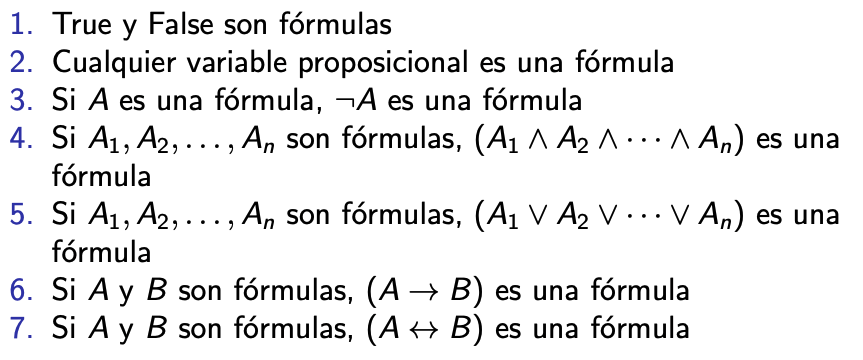
\includegraphics[width=\textwidth]{FBF}
	
	\subsubsection{Pregunta A}
	\begin{enumerate}[label=(\alph*)]
		\item $(p \neg q)$ no es una fórmula bien formada.
		\item $p \vee q \wedge True$ no es una fórmula bien formada pues da lugar a ambigüedad por la falta de paréntesis.
		\item $p \vee q \wedge True$ no es una fórmula bien formada pues da lugar a ambigüedad por la falta de paréntesis.
		\item $\neg (p)$ no es una fórmula bien formada pues el paréntesis es redundante.
		\item $(p \vee \neg q \wedge q)$ no es una fórmula bien formada ya que la falta de paréntesis da lugar a ambigüedad.
		\item $(True \wedge True \wedge True)$ es una formula bien formada.
		\item $(\neg p)$ no es una formula bien formada ya que no hacen falta los paréntesis.
		\item $(p \vee False)$ es una formula bien formada.
		\item $(p = q)$ es una formula bien formada.
	\end{enumerate}
	
	\subsection{Ejercicio 2}
	\begin{enumerate}[label=(\alph*)]
		\item Bien definida
		\item Bien definida
		\item Mal definida. El conector lógico $\vee$ solo acepta variables del tipo Bool pero x e y son $\mathbb{Z}$ 
		\item Bien definida
		\item Mal definida. $(z = 0)$ y $(z = 1)$ no tipa correctamente dado que z es de tipo Bool.
		\item Mal definida. No tipa correctamente dado que $(y < 0)$ es de tipo Bool y la suma solo acepta números.
	\end{enumerate}
	
	\subsection{Ejercicio 3}
	Primero se evalúa $ \alpha = (3+7 = \pi - 8)$ que al ser una igualdad devuelve un valor del tipo Bool. Luego $\alpha \in \{True, False\}$
	y la fórmula resulta $\alpha \wedge True$ que está bien formada.
	
	\subsection{Ejercicio 4}
	Se que $a = True$, $b = True$, $c = True$, $x = False$, $y = False$
	
	\begin{enumerate}[label=(\alph*)]
		\item ($\neg$True $\vee$ True) = False $\vee$ True = True
		\item (True $\vee$ (False $\wedge$ False) $\vee$ True) = (True $\vee$ True $\vee$ True) = True
		\item $\neg$(True $\vee$ False) = $\neg$True = False
		\item ($\neg$(True $\vee$ False)\Iff($\neg$True $\wedge$ $\neg$False)) = ($\neg$True\Iff(False $\wedge$ True)) = (False\Iff False) = True
		\item ((True $\vee$ False)$\wedge$(False $\vee$ True)) = (True $\wedge$ True) = True
		\item ((True $\vee$ False)$\wedge$(False $\vee$ True))\Iff(True $\vee$ (False $\wedge$ False) $\vee$ True), por (e) y (b) respectivamente, cada uno de estos vale True, entonces tenemos True\Iff True = True
		\item ($\neg$ True $\wedge$ $\neg$ False) = (False $\wedge$ True) = False
	\end{enumerate}
	
	Ahora, si $a = False$, $b = False$, $c = False$, $x = True$, $y = True$
	
	\begin{enumerate}[label=(\alph*)]
		\item ($\neg$False $\vee$ False) = True $\vee$ False = True
		\item (False $\vee$ (True $\wedge$ True) $\vee$ False) = (False $\vee$ True $\vee$ False) = True
		\item $\neg$(False $\vee$ True) = $\neg$True = False
		\item ($\neg$(False $\vee$ True)\Iff($\neg$False $\wedge$ $\neg$True)) = ($\neg$True\Iff(True $\wedge$ False)) = (False\Iff False) = True
		\item ((False $\vee$ True)$\wedge$(True $\vee$ False)) = (True $\wedge$ True) = True
		\item ((False $\vee$ True)$\wedge$(True $\vee$ False))\Iff(False $\vee$ (True $\wedge$ True) $\vee$ False), por (d) y (b) respectivamente, cada uno de estos vale True, entonces tenemos True\Iff True = True
		\item ($\neg$ False $\wedge$ $\neg$ True) = (True $\wedge$ False) = False
	\end{enumerate}
	
	\subsection{Ejercicio 5}
	$\bigstar$ Rdo.: Ua fórmula es \textbf{tautología} si siempre toma el valor True, es \textbf{contradicción} si siempre toma el valor False,
	es \textbf{contingencia} si no es ni tautología ni contradicción.
	
	\subsubsection{Inciso A}
	\begin{tabular}{c|c}
		p & (p $\vee$ $\neg$p) \\
		V & V               \\
		V & V               \\
		F & V               \\
		F & V
	\end{tabular}
	
	Es una tautología
	
	\subsubsection{Inciso B}
	\begin{tabular}{c|c}
		p & (p $\wedge$ $\neg$p) \\
		V & F               \\
		F & F
	\end{tabular}
	
	Es una contradicción
	
	\subsubsection{Inciso C}
	\begin{tabular}{c|c|c|c|c}
		p & q & ($\neg$p $\vee$ q) & (p $\rightarrow$ q) & (($\neg$p $\vee$ q) \Iff (p $\rightarrow$ q)) \\
		V & V & V                  & V                   & V                                              \\
		V & F & F                  & F                   & V                                              \\
		F & V & V                  & V                   & V                                              \\
		F & F & V                  & V                   & V                                              \\
	\end{tabular}
	
	Es una tautología. Observar que esto demuestra (p $\rightarrow$ q) = ($\neg$p $\vee$ q) (La Implicación Material)
	
	\subsubsection{Inciso D}
	\begin{tabular}{c|c|c|c}
		p & q & (p $\vee$ q) & ((p $\vee$ q) $\rightarrow$ p) \\
		V & V & V              & V \\
		V & F & V              & V \\
		F & V & V              & F \\
		F & F & F              & V
	\end{tabular}
	
	Es una contingencia.
	
	\subsubsection{Inciso E}
	
	Sean $\alpha$ = $\neg$(p $\wedge$ q); $\beta$ = ($\neg$p $\vee$ $\neg$q)
	
	\begin{tabular}{c|c|c|c|c}
		p & q & $\alpha$ & $\beta$ & $(\alpha \Iff \beta)$\\
		V & V & F & F & V \\
		V & F & V & V & V \\ 
		F & V & V & V & V \\
		F & F & V & V & V 
	\end{tabular}
	
	Es una tautología. Observar que esto demuestra $\neg$(p $\wedge$ q) = ($\neg$p $\vee$ $\neg$q) (La Ley de De Morgan para la conjunción) 
	
	\subsubsection{Inciso F}
	\begin{tabular}{c|c|c|c|c|c|c}
		p & q & $\neg$p & $\neg$q & ($\neg$p $\wedge$ q) & ($\neg$p $\wedge$ $\neg$ q) & (($\neg$p $\wedge$ q)\Iff($\neg$p $\wedge$ $\neg$ q)) \\
		V & V & F & F & F & F & V \\
		V & F & F & V & F & V & F \\
		F & V & V & F & V & V & V \\
		F & F & V & V & F & V & F \\
	\end{tabular}
	
	Es una contingencia.
	
	\subsubsection{Inciso G}
	\begin{tabular}{c|c}
		p & (p $\rightarrow$ p) \\
		V & V\\
		F & V
	\end{tabular}
	
	Es una tautología.
	
	\subsubsection{Inciso H}
	
	\begin{tabular}{c|c|c|c}
		p & q & (p$\wedge$q) & ((p$\wedge$q)$\rightarrow$p) \\
		V & V & V & V \\
		V & F & F & V \\
		F & V & F & V \\
		F & F & F & V \\
	\end{tabular}
	
	Es una tautología.
	
	\subsubsection{Inciso I}
	
	\begin{tabular}{c|c|c|c|c|c|c|c|c}
		p & q & r & (q$\vee$r) & (p $\wedge$ (q$\vee$r)) & (p$\wedge$q) & (p$\wedge$r) & ((p$\wedge$q)$\vee$(p$\wedge$r)) & ((p $\wedge$ (q$\vee$r))\Iff((p$\wedge$q)$\vee$(p$\wedge$r)))\\
		V & V & V & V & V & V & V & V & V \\
		V & V & F & V & V & V & F & V & V \\
		V & F & V & V & V & F & V & V & V \\
		V & F & F & F & F & F & F & F & V \\
		F & V & V & V & F & F & F & F & V \\
		F & V & F & V & F & F & F & F & V \\
		F & F & V & V & F & F & F & F & V \\
		F & F & F & F & F & F & F & F & V \\
	\end{tabular}
	
	Es una tautología. Observar que esto demuestra que p$\wedge$(q$\vee$r) = (p$\wedge$q)$\vee$(p$\wedge$r) (La propiedad distributiva para la conjunción)
	
	\subsubsection{Inciso J}
	
	Sean $\alpha = (q\rightarrow r)$ ; $\beta = (p \rightarrow q)$ ; $\sigma = (p \rightarrow r)$
	
	\begin{tabular}{c|c|c|c|c|c|c|c|c}
		p & q & r & $\alpha$ & $(p \rightarrow \alpha)$ & $\beta$ & $\sigma$ & $(\beta \rightarrow \sigma)$ & $((p \rightarrow \alpha) \rightarrow (\beta \rightarrow \sigma))$\\
		V & V & V & V & V & V & V & V & V \\
		V & V & F & F & F & V & F & F & V \\
		V & F & V & V & V & F & V & V & V \\
		V & F & F & V & V & F & F & V & V \\
		F & V & V & V & V & V & V & V & V \\
		F & V & F & F & V & V & V & V & V \\
		F & F & V & V & V & V & V & V & V \\
		F & F & F & V & V & V & V & V & V
	\end{tabular}
	
	Es una tautología.
	
	\subsection{Ejercicio 6}
	\begin{enumerate}[label=(\alph*)]
		\item $\emph{False}$ es más fuerte que $\emph{True}$.
		\item $(p \wedge q)$ es más fuerte que $(p \vee q)$.
		\item $\emph{True}$ es más fuerte que $\emph{True}$.
		\item $(p \wedge q)$ es más fuerte que $p$.
		\item $\emph{False}$ es más fuerte que $\emph{False}$.
		\item $p$ es más fuerte que $(p\vee q)$.
		\item No hay relación de fuerza.
		\item No hay relación de fuerza.
	\end{enumerate}
	
	\subsection{Ejercicio 7}
	$\emph{False}$ es la m\'as fuerte,  $\emph{True}$ la m\'as d\'ebil
	\subsection{Ejercicio 8}
	\begin{enumerate}[label=(\alph*)]
		\item 
		\begin{tabular}{c|c}
			p & (False $\wedge$ p)\\
			V & F\\
			F & F\\
		\end{tabular}
		(False $\wedge$ p)$\equiv$False (Dominaci\'on de la conjunci\'on)
		\item 
		\begin{tabular}{c|c}
			p & (True $\vee$ p)\\
			V & V\\
			F & V\\
		\end{tabular}
		(True $\vee$ p)$\equiv$False (Dominaci\'on de la disyunci\'on)
		\item 
		\begin{tabular}{c|c}
			p & (True $\wedge$ p)\\
			V & V\\
			F & F\\
		\end{tabular}
		(True $\wedge$ p)$\equiv$p (Neutro de la conjunci\'on)
		\item 
		\begin{tabular}{c|c}
			p & (False $\vee$ p)\\
			V & V\\
			F & V\\
		\end{tabular}
		(True $\vee$ p)$\equiv$p (Neutro de la disyunci\'on)
		\item 
		\begin{tabular}{c|c}
			p & (p $\wedge$ p)\\
			V & V\\
			F & F\\
		\end{tabular}
		(p $\wedge$ p)$\equiv$p (Idempotencia de la conjunci\'on)
		\item 
		\begin{tabular}{c|c}
			p & (p $\vee$ p)\\
			V & V\\
			F & F\\
		\end{tabular}
		(p $\vee$ p)$\equiv$p (Idempotencia de la disyunci\'on)
		\item 
		\begin{tabular}{c|c|c}
			p & $\neg$p &(p $\vee$ $\neg$p)\\
			V & F & V\\
			F & V & V\\
		\end{tabular}
		(p $\vee$ $\neg$p)$\equiv$True (Inversa de la disyunci\'on)
		\item 
		\begin{tabular}{c|c|c}
			p & $\neg$p &(p $\wedge$ $\neg$p)\\
			V & F & F\\
			F & V & F\\
		\end{tabular}
		(p $\wedge$ $\neg$p)$\equiv$False (Inversa de la conjunci\'on)
		\item 
		\begin{tabular}{c|c|c}
			p & $\neg$p & $\neg$$\neg$p\\
			V & F & V\\
			F & V & F\\
		\end{tabular}
		$\neg$$\neg$p$\equiv$p (Doble negaci\'on)
		\item 
		\begin{tabular}{c|c|c|c}
			p & q & (p$\vee$q) & (p$\wedge$(p$\vee$q))\\
			V & V & V & V\\
			V & F & V & V\\
			F & V & V & F\\
			F & F & F & F\\
		\end{tabular}
		(p$\wedge$(p$\vee$q))$\equiv$p (Absorción de la conjunción)
		\item 
		\begin{tabular}{c|c|c|c}
			p & q & (p$\wedge$q) & (p$\vee$(p$\wedge$q))\\
			V & V & V & V\\
			V & F & F & V\\
			F & V & F & F\\
			F & F & F & F\\
		\end{tabular}
		(p$\vee$(p$\wedge$q))$\equiv$p (Absorción de la disyunción)
		\item Probado en 5.E
		$\neg$(p$\wedge$q)$\equiv$($\neg$p$\wedge$$\neg$q) (Ley de De Morgan para la conjunción)
		\item 
		\begin{tabular}{c|c|c|c|c|c|c}
			p & q & (p$\vee$q) & $\neg$(p$\vee$q) & $\neg$p & $\neg$q & ($\neg$p$\wedge$$\neg$q)\\
			V & V & V & F & F & F & F \\
			V & F & V & F & F & V & F \\
			F & V & V & F & V & F & F \\
			F & F & F & V & V & V & V \\
		\end{tabular}
		$\neg$(p$\vee$q)$\equiv$($\neg$p$\wedge$$\neg$q) (Ley de De Morgan para la disyunción)
		\item
		(p$\wedge$q)$\equiv$(q$\wedge$p) (Conmutatividad para la conjunción)
		\item
		(p$\vee$q)$\equiv$(q$\vee$p) (Conmutatividad para la disyunción)
		\item 
		\begin{tabular}{c|c|c|c|c|c|c}
			p & q & r & (q $\wedge$ r) & (p$\wedge$(q $\wedge$ r)) & (p$\wedge$q) & ((p$\wedge$q)$\wedge$r)\\
			V & V & V & V & V & V & V \\
			V & V & F & F & F & V & F \\
			V & F & V & F & F & F & F \\
			V & F & F & F & F & F & F \\
			F & V & V & V & F & F & F \\
			F & V & F & F & F & F & F \\
			F & F & V & F & F & F & F \\
			F & F & F & F & F & F & F \\
		\end{tabular}
		(p$\wedge$(q $\wedge$ r))$\equiv$((p$\wedge$q)$\wedge$r) (Asociatividad de la conjunción)
		\item 
		\begin{tabular}{c|c|c|c|c|c|c}
			p & q & r & (q $\vee$ r) & (p$\vee$(q $\vee$ r)) & (p$\vee$q) & ((p$\vee$q)$\vee$r)\\
			V & V & V & V & V & V & V \\
			V & V & F & V & V & V & V \\
			V & F & V & V & V & V & V \\
			V & F & F & F & V & V & V \\
			F & V & V & V & V & V & V \\
			F & V & F & V & V & V & V \\
			F & F & V & V & V & F & V \\
			F & F & F & F & F & F & F \\
		\end{tabular}
		(p$\vee$(q $\vee$ r))$\equiv$((p$\vee$q)$\vee$r) (Asociatividad de la disyunción)
		\item Probado en 5.I (Distributividad de la conjunción)
		\item 
		\begin{tabular}{c|c|c|c|c|c|c|c}
			p & q & r & (q $\wedge$ r) & (p$\vee$(q $\wedge$ r)) & (p$\vee$q) &  (p$\vee$r) & ((p$\vee$q)$\wedge$(p$\vee$r))\\
			V & V & V & V & V & V & V & V\\
			V & V & F & F & V & V & V & V\\
			V & F & V & F & V & V & V & V\\
			V & F & F & F & V & V & V & V\\
			F & V & V & V & V & V & V & V\\
			F & V & F & F & F & V & F & F\\
			F & F & V & F & F & F & V & F\\
			F & F & F & F & F & F & F & F\\
		\end{tabular}\\
		(p$\vee$(q $\wedge$ r))$\equiv$((p$\vee$q)$\wedge$(p$\vee$r)) (Distibutividad de la disyunción)
		\item 
		\begin{tabular}{c|c|c|c|c|c}
			p & q & (p$\rightarrow$q) & $\neg$p & $\neg$q & ($\neg$q$\rightarrow$$\neg$p)\\
			V & V & V & F & F & V\\
			V & F & F & F & V & F\\
			F & V & V & V & F & V\\
			F & F & V & V & V & V\\
		\end{tabular}
		(p$\rightarrow$q)$\equiv$($\neg$q$\rightarrow$$\neg$p) (Contraposición lógica)
		\item Probado en 5.C (Implicación Material)
		\item 
		\begin{tabular}{c|c|c|c|c|c}
			p & q & (p\Iff q) & (p$\rightarrow$q) & (q$\rightarrow$p) & ((p$\rightarrow$q)$\wedge$(q$\rightarrow$p))\\
			V & V & V & V & V & V\\
			V & F & F & F & V & F\\
			F & V & F & V & F & F\\
			F & F & V & V & V & V\\
		\end{tabular}
		(p\Iff q)$\equiv$((p$\rightarrow$q)$\wedge$(q$\rightarrow$p)) (Equivalencia material)
	\end{enumerate}
	
	\subsection{Ejercicio 9}
	
		\subsubsection{Inciso A}
		((p$\wedge$p)$\vee$p) $\equiv$ (Idempotencia de la conjunción)\\
		(p$\vee$p) $\equiv$ (Idempotencia de la disyunción)\\
		 p
		 
		 \subsubsection{Inciso B}
		 $\neg$($\neg$p$\vee$$\neg$q) $\equiv$ (Ley de De Morgan para la disyunción)\\
		 ($\neg$$\neg$p$\wedge$$\neg$$\neg$q) $\equiv$ (Doble negación)\\
		 (p $\wedge$ q)
	
		\subsubsection{Inciso C}
		( ( (p $\wedge$ ($\neg$p$\vee$q)) $\vee$ q ) $\vee$ (p $\wedge$ (p$\vee$q)) ) $\equiv$ (Distributiva para la conjunción)\\
		( ( ((p $\wedge$$\neg$p) $\vee$ (p$\wedge$q)) $\vee$ q) $\vee$ (p$\wedge$(p$\vee$q))) $\equiv$ (Inversa de la conjunción, Asociatividad de la conjunción, Absorción de la conjunción)\\
		( ( (False $\vee$ (p$\wedge$q) $\vee$ q) $\vee$ p)) $\equiv$ (Absorción de la disyunción)\\
		( ( False $\vee$ q ) $\vee$ p) $\equiv$ (Neutro de la disyunción)\\
		(q $\vee$ p)
		
		\subsubsection{Inciso D}
		($\neg$p $\rightarrow$ $\neg$(p$\rightarrow$$\neg$q)) $\equiv$ (Implicación Material)\\
		($\neg$p $\rightarrow$ $\neg$($\neg$p$\vee$$\neg$q)) $\equiv$ (Ley de De Morgan para la conjunción)\\
		($\neg$p $\rightarrow$ ($\neg$$\neg$p$\wedge$$\neg$$\neg$q)) $\equiv$ (Doble negación)\\
		($\neg$p $\rightarrow$ (p$\wedge$q)) $\equiv$ (Implicación Material)\\
		($\neg$$\neg$p $\vee$ (p$\wedge$q)) $\equiv$ (Doble Negación)\\
		(p $\vee$ (p$\wedge$q)) $\equiv$ (Absorción de la disyunción)\\
		p
		
		\subsubsection{Inciso E}
		(((p$\rightarrow$q) $\wedge$ (p$\wedge$$\neg$q))$\rightarrow$q) $\equiv$ (Implicación Material)\\
		((($\neg$p$\vee$q) $\wedge$ (p$\wedge$$\neg$q))$\rightarrow$q) $\equiv$ (Asociatividad de la conjunción, Distributividad de la conjunción)\\
		((((p$\wedge$$\neg$p) $\vee$ (p$\wedge$q)) $\wedge$ $\neg$q)$\rightarrow$q) $\equiv$ (Inversa de la conjunción)\\
		(((False $\vee$ (p$\wedge$q)) $\wedge$ $\neg$q)$\rightarrow$q) $\equiv$ (Neutro de la disyunción)\\
		(((p$\wedge$q) $\wedge$ $\neg$q)$\rightarrow$q) $\equiv$ (Asociatividad de la conjunción)\\
		((p $\wedge$ (q$\wedge$$\neg$q))$\rightarrow$q) $\equiv$ (Inversa de la conjunción)\\
		((p $\wedge$ False)$\rightarrow$q) $\equiv$ (Dominación de la conjunción)\\
		(False$\rightarrow$q) $\equiv$ (Implicación Material)\\
		($\neg$False $\vee$ q) $\equiv$ (True $\vee$ q) $\equiv$ (Dominación de la disyunción)\\
		True
		
		\subsubsection{Inciso F}
		$\neg$($\neg$(p $\wedge$ q) $\vee$ (p $\vee$ q))$\rightarrow$($\neg$$\neg$p $\vee$ $\neg$p) $\equiv$ (Doble negación, Ley de De Morgan para la conjunción)\\
		$\neg$(($\neg$p $\vee$ $\neg$q) $\vee$ p $\vee$ q)$\rightarrow$(p $\vee$ $\neg$p) $\equiv$ (Inversa de la disyunción, Asociatividad de la disyunción)\\
		$\neg$(($\neg$p $\vee$ p) $\vee$ ($\neg$q $\vee$ q))$\rightarrow$True $\equiv$ (Inversa de la disyunción)\\
		$\neg$(True $\vee$ True)$\rightarrow$True $\equiv$\\
		False $\rightarrow$ True $\equiv$\\
		True
	\subsection{Ejercicio 10}
	
		\subsubsection{Inciso A}
		((p$\wedge$p)$\wedge$p)$\rightarrow$p $\equiv$ (Idempotencia de la conjunción,Asociatividad de la conjunción)\\
		p$\rightarrow$p $\equiv$ (Implicación material)\\
		($\neg$ p $\vee$ p) $\equiv$ (Inversa disyunción)\\
		True\\
		
		Por lo tanto ((p$\wedge$p)$\wedge$p)$\rightarrow$p $\equiv$ True
		
		\subsubsection{Inciso B}
		(($\neg$p$\vee$$\neg$q)$\vee$(p$\wedge$q)$\rightarrow$(p$\wedge$q)) $\equiv$ (Asociatividad de la disyunción, Distributividad de la disyunción)\\
		(($\neg$p$\vee$$((\neg$q$\vee$p)$\wedge$($\neg$q$\wedge$q)))$\rightarrow$(p$\wedge$q)) $\equiv$ (Inversa de la disyunción)\\
		(($\neg$p$\vee$$((\neg$q$\vee$p)$\wedge$True))$\rightarrow$(p$\wedge$q)) $\equiv$ (Neutro de la conjunción)\\
		(($\neg$p$\vee$$(\neg$q$\vee$p))$\rightarrow$(p$\wedge$q)) $\equiv$ (Asociatividad de la disyunción)\\
		(($\neg$p$\vee$p)$\vee$$\neg$q)$\rightarrow$(p$\wedge$q)) $\equiv$ (Inversa de la disyunción)\\
		(True$\vee$$\neg$q)$\rightarrow$(p$\wedge$q)) $\equiv$ (Dominación de la disyunción)\\
		(True$\rightarrow$(p$\wedge$q)) $\equiv$ (Implicación material)\\
		($\neg$True$\vee$(p$\wedge$q)) $\equiv$ (False$\vee$(p$\wedge$q)) $\equiv$ (Neutro de disyunción)\\
		(p $\wedge$ q)\\
		
		Por lo tanto (($\neg$p$\vee$$\neg$q)$\vee$(p$\wedge$q)$\rightarrow$(p$\wedge$q)) $\equiv$ (p $\wedge$ q)
		
		\subsubsection{Inciso C}
		($\neg$p$\rightarrow$(q$\wedge$r)) $\equiv$ (Implicación material, Doble negación)\\
		(p$\vee$(q$\wedge$r)) $\equiv$ (Distributividad de la disyunción)\\
		((p$\vee$q)$\wedge$(p$\vee$r))\\
		
		Por lo tanto ($\neg$p$\rightarrow$(q$\wedge$r)) $\equiv$ ((p$\vee$q)$\wedge$(p$\vee$r))
		
		\subsubsection{Inciso D}
		$\neg$($\neg$p)$\rightarrow$($\neg$($\neg$p$\wedge$$\neg$q)) $\equiv$ (Ley de De Morgan para la conjunción, Doble negación)\\
		p$\rightarrow$(p $\vee$ q) $\equiv$ (Implicación material,Doble negación)\\
		($\neg$ p$\vee$(p$\vee$q)) $\equiv$ (Asociatividad de la disyunción, Inversa de la disyunción)\\
		(True $\wedge$ q) $\equiv$ (Dominación de la disyunción)\\
		True\\
		
		Por lo tanto $\neg$($\neg$p)$\rightarrow$($\neg$($\neg$p$\wedge$$\neg$q)) $\not\equiv$ q
		
		\subsubsection{Inciso E}
		((True $\wedge$ p)$\vee$($\neg$p$\vee$False)$\rightarrow$$\neg$($\neg$p$\vee$q)) $\equiv$ (Neutro de la conjunción, Neutro de la disyunción, Ley de De Morgan para la disyunción, Doble negación)\\
		((p$\vee$$\neg$p)$\rightarrow$(p$\wedge$$\neg$q)) $\equiv$ (Inversa de la conjunción)\\
		(False $\rightarrow$ (p $\wedge$$\neg$q)) $\equiv$ (Implicación Material)\\
		True $\vee$ (p $\wedge$$\neg$q)) $\equiv$ (Dominación de la disyunción)\\
		True\\
		
		Por lo tanto ((True $\wedge$ p)$\vee$($\neg$p$\vee$False)$\rightarrow$$\neg$($\neg$p$\vee$q)) $\not\equiv$ (p$\wedge$$\neg$q)
		
		\subsubsection{Inciso F}
		(p$\vee$($\neg$p$\wedge$q)) $\equiv$ (Distributiva de la disyunción)\\
		((p$\vee$$\neg$p)$\wedge$(p$\vee$q)) $\equiv$ (Inversa de la disyunción)\\
		(True$\wedge$(p$\vee$q)) $\equiv$ (Neutro de la conjunción)\\
		(p$\vee$q) $\equiv$ (Implicación Material)\\
		($\neg$p$\rightarrow$q)\\
		
		Por lo tanto, (p$\vee$($\neg$p$\wedge$q)) $\equiv$ ($\neg$p$\rightarrow$q)
		
		\subsubsection{Inciso G}
		$\neg$(p$\wedge$(q$\wedge$s)) $\equiv$ (Asociatividad de la conjunción)\\
		$\neg$(p$\wedge$q$\wedge$s) $\equiv$ (Ley de De Morgan para la conjunción)\\
		($\neg$p$\vee$$\neg$q$\vee$$\neg$s) $\equiv$ (Implicación Material)\\
		s$\rightarrow$($\neg$p$\vee$$\neg$q)\\
		
		Por lo tanto $\neg$(p$\wedge$(q$\wedge$s)) $\equiv$ s$\rightarrow$($\neg$p$\vee$$\neg$q)
		
		\subsubsection{Inciso H}
		(p$\rightarrow$(q$\wedge$$\neg$(q$\rightarrow$r))) $\equiv$ (Implicación Material)\\
		($\neg$p$\vee$(q$\wedge$$\neg$($\neg$q$\vee$r))) $\equiv$ (Ley de De Morgan para la disyunción, Doble negación)\\
		($\neg$p$\vee$(q$\wedge$(q$\wedge$$\neg$r))) $\equiv$ (Distributiva para la disyunción)\\
		(($\neg$p$\vee$q)$\wedge$($\neg$p$\vee$(q$\wedge$$\neg$r)))\\
		
		Por lo tanto, (p$\rightarrow$(q$\wedge$$\neg$(q$\rightarrow$r))) $\equiv$ (($\neg$p$\vee$q)$\wedge$($\neg$p$\vee$(q$\wedge$$\neg$r)))
		
	\subsection{Ejercicio 11}
		\subsubsection{Inciso A}
		Arranquemos probando que la conjunción es expresable mediante la negación y la disyunción. Propongo ver que (p$\wedge$q) $\equiv$ $\neg$($\neg$p$\vee$$\neg$q)\\
		\begin{tabular}{c|c|c|c|c|c|c}
			p & q & (p$\wedge$q) & $\neg$p & $\neg$q & ($\neg$p$\vee$$\neg$q) & $\neg$($\neg$p$\vee$$\neg$q)\\
			V & V & V & F & F & F & V\\
			V & f & F & F & V & V & F\\
			V & V & F & V & F & V & F\\
			V & V & F & V & V & V & F\\
		\end{tabular}
		
		\subsubsection{Inciso B}
		Como ya sabemos, (p$\rightarrow$q) $\equiv$ ($\neg$p $\vee$ q)  (Probado en 5.E)
		
		\subsubsection{Inciso C}
		Luego, como probamos que (p\Iff q) $\equiv$ ((p$\rightarrow$q)$\wedge$(q$\rightarrow$p)) en 8.U, y tanto ($\rightarrow$) como ($\wedge$) son expresables mediante negaciones y disyunciones, (\Iff)  también lo es
	\subsection{Ejercicio 12}
		\subsubsection{Inciso A}
		\begin{itemize}
			\item ($\emph{f}$ $\rightarrow$ $\neg$($\emph{e}$\Iff $\emph{m}$))
			\item ($\neg$$\emph{f}$ $\rightarrow$ $\neg$$\emph{e}$)
			\item (($\emph{e}$$\wedge$$\emph{f}$) $\rightarrow$ $\emph{m}$)
		\end{itemize}
		\subsubsection{Inciso B}
		Sabemos que si no es fin de semana, Juan no estudia (por el segundo item del Inciso A). Pero a la vez por el primer item, vemos que si es fin de semana, existe la posibilidad de que Juan estudie, siempre y cuando él no este escuchando música, ahora, el tercer item nos dice que si estudia y es fin de semana, escuchará música, lo cual haría incumplir el 1er item.
		Queda pendiente la verificación con lógica, pero creería que juntar las 3 proposiciones lleva a una contradicción.
	
	\subsection{Ejercicio 13}
		Defino $j = \text{Conocen a Juan; } c = \text{Conocen a Camila; } g = \text{Conocen a Gonzalo}$ \\
		
		\begin{tabular}{c|c|c|c|c|c|c|c}
			j & c & g & (j $\rightarrow$ c) & (c $\rightarrow$ g) & ((j $\rightarrow$ c)$\vee$(c $\rightarrow$ g)) & (j $\rightarrow$ g) & (((j $\rightarrow$ c)$\vee$(c $\rightarrow$ g))$\rightarrow$(j $\rightarrow$ g)) \\
			F          & F          & F          & V              & V              & V                          & V              & V                                      \\
			F          & F          & V          & V              & V              & V                          & V              & V                                      \\
			F          & V          & F          & V              & F              & F                          & V              & V                                      \\
			F          & V          & V          & V              & V              & V                          & V              & V                                      \\
			V          & F          & F          & F              & V              & F                          & F              & V                                      \\
			V          & F          & V          & F              & V              & F                          & V              & V                                      \\
			V          & V          & F          & V              & F              & F                          & F              & V                                      \\
			V          & V          & V          & V              & V              & V                          & V              & V                                     
		\end{tabular}\\
		Luego es cierto que si todos conocen a Juan entonces todos conocen a Gonzalo
	
	\subsection{Ejercicio 14}
		Si p = pelea y o = ojo morado. Luego se que $p \rightarrow o$ pero si o es verdadero, puede pasar que p sea True o que sea False indistintamente. Por ejemplo si digo "Si llueve, hay nubes negras", y luego afirmo que hay nubes negras, eso no quiere decir que esté lloviendo
		Esto es llamado falacia del consecuente
		
	\subsection{Ejercicio 15}
		\begin{enumerate}[label=(\alph*)]
			\item True
			\item True
			\item $\perp$
			\item $\perp$
			\item $\perp$
			\item $\perp$ 
		\end{enumerate}
	\subsection{Ejercicio 16}
		El operador $\implicaLuego$ se evalúa de forma secuencial, de izquierda a derecha, y es usado en lógica ternaria. Su tabla de verdad es:\\
		\begin{tabular}{c|c|c|c}
			p & q & p$\rightarrow$q & p$\implicaLuego$q\\
			V & V & V & V\\
			V & F & F & F\\
			F & V & V & V\\
			F & F & V & V\\
			V & $\perp$ & - & $\perp$\\
			F & $\perp$ & - & V\\
			$\perp$ & V & - & $\perp$\\
			$\perp$ & F & - & $\perp$\\
			$\perp$ & $\perp$ & - & $\perp$\\
		\end{tabular}
	\subsection{Ejercicio 17}
		El operador $\yLuego$ se evalúa de forma secuencial, de izquierda a derecha, y es usado en lógica ternaria. Su tabla de verdad es:\\
		\begin{tabular}{c|c|c|c}
			p & q & p$\wedge$q & p$\yLuego$q\\
			V & V & V & V\\
			V & F & F & F\\
			F & V & F & F\\
			F & F & F & F\\
			V & $\perp$ & - & $\perp$\\
			F & $\perp$ & - & F\\
			$\perp$ & V & - & $\perp$\\
			$\perp$ & F & - & $\perp$\\
			$\perp$ & $\perp$ & - & $\perp$\\
		\end{tabular}
	\subsection{Ejercicio 18}
		El operador $\oLuego$ se evalúa de forma secuencial, de izquierda a derecha, y es usado en lógica ternaria. Su tabla de verdad es:\\
		\begin{tabular}{c|c|c|c}
			p & q & p$\vee$q & p$\oLuego$q\\
			V & V & V & V\\
			V & F & V & V\\
			F & V & V & V\\
			F & F & F & F\\
			V & $\perp$ & - & V\\
			F & $\perp$ & - & $\perp$\\
			$\perp$ & V & - & $\perp$\\
			$\perp$ & F & - & $\perp$\\
			$\perp$ & $\perp$ & - & $\perp$\\
		\end{tabular}
	\subsection{Ejercicio 19}
		$b=c=True, a=False, x=y=\perp$
		\begin{enumerate}[label=(\alph*)]
		\item $(\neg x \oLuego b) \equiv (\neg \perp \oLuego True) \equiv \perp$
		\item $((c \yLuego (y \yLuego a))\oLuego b) \equiv (True \oLuego(\perp \yLuego False)\oLuego True) \equiv (True \oLuego \perp \oLuego True) \equiv True$
		\item $\neg (c \oLuego y) \equiv \neg (True \oLuego \perp) \equiv \neg True \equiv True$
		\item $(\neg(True \oLuego \perp)\Iff(\neg True \yLuego \neg \perp)) \equiv (\neg True \Iff False) \equiv (False \Iff False) \equiv True$
		\item $((True \oLuego \perp) \yLuego (False \oLuego True)) \equiv (True \yLuego True) \equiv True$
		\item $(True \Iff True) \equiv True$
		\item $(\neg True \yLuego \neg \perp) \equiv (False \yLuego \perp) \equiv False$
		\end{enumerate}
	\subsection{Ejercicio 20}
		$p=True, q=False, r=\perp$
		\begin{enumerate}[label=(\alph*)]
		\item $(True \yLuego True) \equiv True$
		\item $(False \implicaLuego (True \yLuego False)) \equiv (False \implicaLuego False) \equiv True$
		\item $(True \implicaLuego (True \oLuego \perp)) \equiv (True \implicaLuego True)  \equiv True$
		\item $(False \oLuego (\perp \yLuego (False \yLuego True))) \equiv (False \oLuego (\perp \yLuego False)) \equiv (False \oLuego \perp) \equiv \perp$
		\item $((True \yLuego False)\yLuego \perp) \equiv (False \yLuego \perp) \equiv False$
		\item $((True \oLuego False)\oLuego \perp) \equiv (True \oLuego \perp) \equiv True$
		\item $((True\yLuego False)\yLuego((False \implicaLuego False)\oLuego(T\implicaLuego(False \yLuego \perp)))) \equiv (\perp \yLuego (True \oLuego False)) \equiv \perp$
		\item $((True \yLuego \neg False)\implicaLuego False) \equiv (True \implicaLuego False) \equiv False$
		\item $(True \yLuego(False \Iff False)) \equiv (True \yLuego True) \equiv True$
		\item $(\neg (True \oLuego \perp)\implicaLuego \perp) \equiv (False \implicaLuego \perp) \equiv True$
		\item $((True \implicaLuego \perp)\Iff(True \yLuego (True \yLuego \neg False))) \equiv (\perp \Iff False) \equiv \perp$
		\item $((True \implicaLuego (False \implicaLuego \perp))\implicaLuego((True \implicaLuego False)\implicaLuego(True\implicaLuego \perp))) \equiv (True \implicaLuego (False \implicaLuego \perp)) \equiv (True \implicaLuego True) \equiv True$
		\end{enumerate}
	\subsection{Ejercicio 21}
		TODO
\end{document}
